\chapter{Ordinary Differential Equations}
\minitoc

In this chapter you'll learn about a mathematical tool for describing physical systems, differential equations, and two computation tools for solving them, Euler's method and {\tt ode45}.


\section{Differential Equations}
\label{diffeq}

A {\emph differential equation} (DE) is an equation that describes the
derivatives of an unknown function.  ``Solving a DE'' means finding a
function whose derivatives satisfy the equation.

\index{differential equation}
\index{equation!differential}

For example, suppose we would like to predict the population of yeast growing in a nutrient solution.  Assume that we know the initial population is 5 billion yeast cells.

When yeast grow in particularly yeast-friendly
conditions, the rate of growth at any point in time is proportional to
the current population.

If we define $y(t)$ to be the population at 
time $t$, we can write the following equation for the rate of growth:
%
\begin{equation}
\frac{dy}{dt}(t) = a y(t)
\end{equation}
%
where $\frac{dy}{dt}(t)$ is the derivative of $y(t)$ and
$a$ is a constant that characterizes how quickly the population
grows.
This equation is ``differential'' because it relates a function to one of its derivatives.

\index{ordinary differential equation}

It is an {\emph ordinary} differential equation (ODE) because all the
derivatives involved are taken with respect to the
same variable.
If it related derivatives with respect to
different variables (partial derivatives), it would be a {\emph partial}
differential equation.

\index{first-order differential equation}

This equation is {\emph first-order} because it involves only first
derivatives.  If it involved second derivatives, it would be second order,
and so on.

\index{linear differential equation}

Lastly, it's {\bf linear} because each term involves $t$, $f$, or
$df/dt$ raised to the first power; if any of the terms involved
products or powers of $t$, $f$, and $df/dt$ it would be
nonlinear.

Now suppose we want to predict the yeast population in the future.  We can do that using Euler's method.

\section{Euler's Method}

Here's a test to see if you're as smart as Euler.  Let's say you arrive at time $t$ and measure the current population, $y$, and
the rate of change, $r$.  What do you think the population will
be after some period of time $\Delta t$ has elapsed?

If you said $y + r \Delta t$, congratulations!  You just invented
Euler's method.

\index{Euler's Method}

This estimate is based on the assumption that $r$ is constant, but
in general it's not, so we only expect the estimate to be good if
$r$ changes slowly and $\Delta t$ is small. So what if we want to make a prediction when $\Delta t$ is large?
One option is to break $\Delta t$ into smaller pieces, called
{\emph time steps}. Then we can use the following equations to get from one time step to the next:

\begin{eqnarray}
T_{i+1} &=& T_i + dt                       \\
Y_{i+1} &=& Y_i + \frac{df}{dt}(t)~dt          
\end{eqnarray}

Here $\{T_i\}$ is a sequence of times where we estimate the value
of $y$, and $\{Y_i\}$ is the sequence of estimates.  For each
index $i$, $Y_i$ is an estimate of $y(T_i)$.

\index{time step}

If the rate doesn't change too fast and the time step isn't
too big, Euler's method is accurate enough for most purposes.  One
way to check is to run it once with time step $dt$ and then run it
again with time step $dt/2$.  If the results are the same, they are
probably accurate, as . . .; otherwise, we can cut the time step again.


\section{Implementing Euler's method}

As an example I'll use Euler's method to solve the equation from Section~\ref{diffeq}:

\[ \frac{dy}{dt}(t) = a y(t) \]

with the initial condition $y(0) = 5$ billion cells and
the growth parameter $a = 0.2$ per hour. 

\index{top-level function}

As a first step, I created a file named {\emph euler.m} with a top-level function and a helper function:

\begin{code}
function res = euler()
    T(1) = 0;
    Y(1) = 5;
    r = rate_func(T(1), Y(1))
end

function res = rate_func(t, y)
   a = 0.2;
   dydt = a * y;
   res = dydt;
end
\end{code}

In {\tt euler} I initialize the initial conditions and then call \verb"rate_func".  In \verb"rate_func" I compute the rate of change in the population.

\index{initial condition}

After testing these functions, I added code to {\tt euler} to implement these difference equations:

\begin{eqnarray}
T_{i+1} &=& T_i + \Delta t             \\
Y_{i+1} &=& Y_i + r \Delta t           \\
\end{eqnarray}
%
where $r$ is the rate of population growth computed by \verb"rate_func".
Listing~\ref{lst:euler_method} has the code we need:

\begin{lstlisting}[caption={A function implementing Euler's method}, label={lst:euler_method}]
function res = euler()
    T(1) = 0;
    Y(1) = 5;
    dt = 0.1;
    
    for i=1:100
        r = rate_func(T(i), Y(i));
        T(i+1) = T(i) + dt;
        Y(i+1) = Y(i) + r * dt;
    end
    plot(T, Y)
end
\end{lstlisting}

...

If we run the code, we should get a plot of population over time, shown in Figure~\ref{fig:euler}. 

\begin{figure}[ht]
\centerline{\includegraphics[height=3in]{book/figs/euler.eps}}
\caption{Solution to a simple differential equation by Euler's method.}
\label{fig:euler}
\end{figure}

As you can see, the population doubles in a little less than 4 hours.


\section{Improving with ode45}
\label{ode45}


A limitation of Euler's method is that it assumes that the derivative is constant between time steps, and that's not generally true.  Fortunately, there are better methods that estimate the derivative between time steps, and they are much more accurate.

\index{time step} 
\index{ode45@{\tt ode45}}

MATLAB provides a function called {\tt ode45} that implements one of these methods.  In this section I'll explain how to use it; you can read more about how it works in Section~\ref{howode45}.

\index{rate function}
\index{function!rate}

In order to use {\tt ode45}, you have to write a function that evaluates $dy/dt$ as a function of $t$ and $y$.  Fortunately, we already have one, \verb"rate_func":

\begin{code}
function res = rate_func(t, y)
   a = 0.2;
   dydt = a * y;
   res = dydt;
end
\end{code}

We can call {\tt ode45} from the Command Window like this:

\begin{code}
[T, Y] = ode45(@rate_func, [0, 4], 5);
plot(T, Y)
\end{code}

The first argument is a function handle, as we saw in Section~\ref{fzero}.  The second argument is the time interval where we want to evaluate the solution; in this case the interval is from $t=0$ to $t=4$ hours.  The third argument is the initial population, 5 billion cells.

\index{function handle}
\index{handle!function}
\index{output variable}
\index{variable!output}

{\tt ode45} is the first function we've seen that returns {\em two} output variables.  In order to store them, we have to assign them to two variables, {\tt T} and {\tt Y}.

\begin{figure}[ht]
\centerline{\includegraphics[height=3in]{book/figs/runge.eps}}
\caption{Solutions to a simple differential equation by Euler's method and {\tt ode45}.}
\label{fig:runge}
\end{figure}

Figure~\ref{fig:runge} shows the results.  The solid line is the estimate we computed with Euler's method; the dashed line is the solution from {\tt ode45}.

For the first 4-5 hours, the two solutions are indistinguishable.  But as the rate of growth increases, Euler's method gets less accurate.

In general, you should use {\tt ode45} instead of Euler's method.  It's almost always more accurate.  


\section{Time Dependence}

Looking at \verb"rate_func" in the previous section, you might notice that it takes {\tt t} as an input variables but doesn't use it.  That's because the growth rate does not depend on time---bacteria don't know what time it is.

\index{time dependence}

But rats do.  Or, at least, they know what season it is.
Suppose that the population growth rate for rats
depends on the current population and the availability of food,
which varies over the course of the year.
The differential equation might be something like
%
\begin{equation}
\frac{dy}{dt}(t) = a y(t) \left(1 - \cos (\omega t) \right)
\end{equation}
%
where $t$ is time in days and $y(t)$ is the population at time $t$.

$a$ and $\omega$ are {\emph parameters}, values that
quantify a physical aspect of the scenario being modeled.  Parameters are often constants, but in some models they vary in time.

\index{parameter}

In this example, $a$ characterizes the reproductive rate per day, and
$\omega$ is the frequency of a periodic function that describes
the effect of varying food supply on reproduction.

We'll use the values $a = 0.002$
and $\omega = 2 \pi/365$ (one cycle per year).
The growth rate is lowest at $t=0$, on January 1, and highest at $t=365/2$, on June 1.

Now we can write a function that evaluates the growth rate:

\begin{code}
function res = rate_func(t, y)
    a = 0.002;
    omega = 2*pi / 365;
    res = a * y * (1 - cos(omega * t));
end
\end{code}

To test this function, I put it in a file called {\emph rats.m} with a top-level function called {\tt rats}:

\begin{code}
function res = rats()
    t = 365/2;
    y = 1000;
    res = rate_func(t, y);
end
\end{code}

Suppose there are 1000 rats at $t=365/2$.  We can compute the growth rate like this:

\begin{code}
>> r = rats

r = 4
\end{code}

So if there are 1000 rats on June 31, we expect them to 
reproduce at a rate that would produce about 4 new rats per day. 

Since the growth rate is constantly changing, it's not easy to predict
the future rat population, but that is exactly what {\tt ode45} does.
Here's how:

\begin{code}
[T, Y] = ode45(@rate_func, [0, 365], 1000)
plot(T, Y)
\end{code}

The first argument is a function handle, again.  The second argument is the interval we are interested
in, one year.  
The third argument is the initial population, $y(0) = 1000$.

\index{interval}
\index{time span}
Figure~\ref{fig:rats} shows the results. 
\begin{figure}[ht]
\centerline{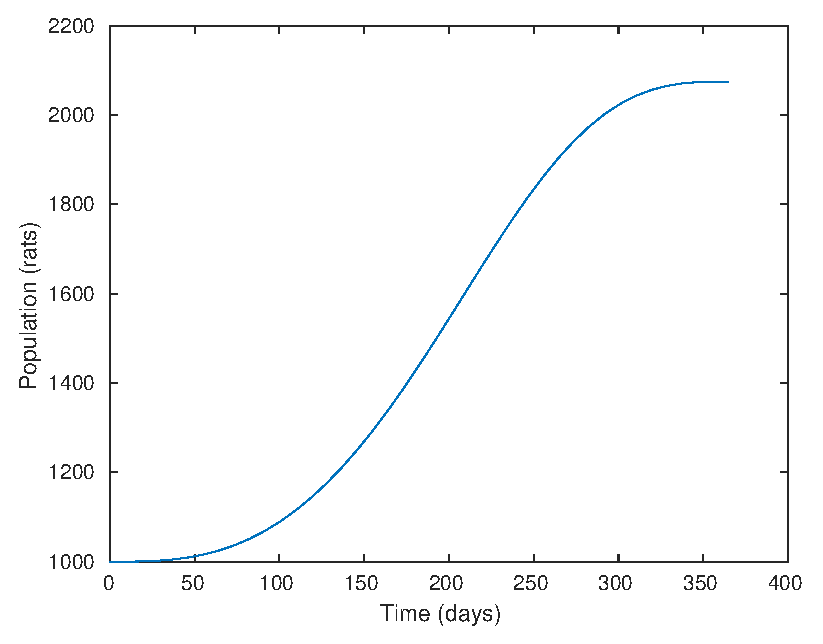
\includegraphics[height=3in]{book/figs/rats.eps}}
\caption{Solutions to a simple differential equation by Euler's method and {\tt ode45}.}
\label{fig:rats}
\end{figure}

The population grows slowly during the winter, quickly during the summer, and the slowly again in the fall.

% TODO

To see the population at the end of the year, you can display the last element of {\tt Y}:

\begin{code}
Y(end)
2.0751e+03
\end{code}

That's a little more than 2000 rats, so the population roughly doubles in one year.

Notice we used {\tt end}, which is a special word in MATLAB; when it appears as an index,
it means ``the index of the last element''.  You can use it in an
expression, so {\tt Y(end-1)} is the second-to-last element of
{\tt Y}.

\index{end@{\tt end}}
\index{index!{\tt end}}


\section{What Could Go Wrong?}

Don't forget the {\tt @} on the function handle.
If you leave it out, MATLAB treats the first argument as a function
call, and calls \verb"rate_func" without providing arguments.

\index{rate function}
\index{function handle}

\begin{code}
Not enough input arguments.

Error in rats>rate_func (line 18)
    res = a * y * (1 - cos(omega * t));

Error in rats (line 6)
    [T, Y] = ode45(rate_func, [0, 365], 1000);
\end{code}

Also, remember that the function you write will be called by
{\tt ode45}, which means the function has to take two input variables, 
{\tt t} and {\tt y}, in that order, and return one output variable, 
{\tt res}.

\index{output variable}

If you're working with a rate function like this:

\begin{equation}
\frac{dy}{dt}(t) = a y(t)
\end{equation}

You might be tempted to write this:

\begin{code}
function res = rate_func(y)        % WRONG
    a = 0.002;
    res = a * y;
end
\end{code}

But that would be wrong.  So very wrong.  Why?  Because
when {\tt ode45} calls {\tt rate\_func}, it provides two arguments.
If you only take one input variable, you'll get an error.  So
you have to write a function that takes {\tt t} as an input
variable, even if you don't use it.

\index{input variable}

\begin{code}
function res = rate_func(t, y)     % RIGHT
    a = 0.002;
    res = a * y;
end
\end{code}

Another common error is to write a function that doesn't make
an assignment to the output variable.  If you write something
like this:

\begin{code}
function res = rate_func(t, y)
    a = 0.002;
    omega = 2*pi / 365;
    r = a * y * (1 - cos(omega * t));    % WRONG
end
\end{code}

And then call it from {\tt ode45}, you get

\begin{code}
Output argument "res" (and maybe others) not assigned during call
to "rate_func".
\end{code}

I hope these warnings save you some time debugging.

\section{Labeling Axes}

The plots in this chapter have labels on the axes, and one of them has a legend, but I didn't show you how to do that. Let's do it now.

\index{labeling axes}
\index{axes}
\index{xlabel@{\tt xlabel}}
\index{ylabel@{\tt ylabel}}

The functions to label the axes are {\tt xlabel} and {\tt ylabel}:

\begin{code}
xlabel('Time (hours)')
ylabel('Population (billions of cells)')
\end{code}

The function to generate a legend is {\tt legend}:

\begin{code}
legend('euler', 'ode45')
\end{code}

\index{legend@{\tt legend}}

The arguments are the labels for the lines, in the order they were drawn.  Usually the legend is in the upper right corner, but you can move it by providing an optional argument called {\tt Location}:

\begin{code}
legend('euler', 'ode45', 'Location', 'northwest')
\end{code}

Finally, I saved the figures using {\tt saveas}:

\begin{code}
saveas(gcf, 'runge.eps', 'epsc')
\end{code}

The first argument is the figure we want to save; {\tt gcf} is a MATLAB command that stands for ``get current figure'', which is the figure we just drew.  The second argument is the filename.  The extension specifies the format we want, which is Encapulated PostScript.  The third argument tells MATLAB what ``driver'' to use.  The details aren't important, but {\tt epsc} generates figures in color.

\index{figure}
\index{get current figure}
\index{gcf@{\tt gcf}}
\index{saveas@{\tt saveas}}

\section{Summary}
...

\section{Glossary}

\begin{description}

\item[differential equation (DE):] An equation that relates the
derivatives of an unknown function.

\item[ordinary DE (ODE):] A DE in which all derivatives are taken with
respect to the same variable.

\item[partial DE (PDE):] A DE that includes derivatives with respect to
more than one variable

\item[first-order DE:] A DE that includes only first derivatives.

\item[linear DE:] A DE that includes no products or powers of the
function and its derivatives.

\item[time step:] The interval in time between successive estimates
in the numerical solution of a DE.

\item[parameter:] A value that appears in a model to quantify some
physical aspect of the scenario being modeled.

\end{description}


\section{Exercises}

\begin{ex}

\index{coffee}
\index{cooling}
\index{Newton's law of cooling}

Suppose that you're given an 8 ounce cup of coffee at \SI{90}{\celsius}.
You have learned from bitter experience that the hottest coffee you
can drink comfortably is \SI{60}{\celsius}.  

If the temperature of the coffee drops by \SI{0.7}{\celsius} during the first minute, how long will you have to wait to drink your coffee?

You can answer this question with Newton's Law of Cooling (See \emph{https://en.wikipedia.org/wiki/Newton's\_law\_of\_cooling}).:
%
\begin{equation*}
\frac{dy}{dt}(t) = -k (y(t) - e)
\end{equation*}
%
where $y(t)$ is the temperature of the coffee at time $t$,
$e$ is the temperature of the environment, and $k$ is a parameter
that characterizes the rate of heat transfer from the coffee from the environment.

Let's assume that $e$ is \SI{20}{\celsius} and constant; that is, the coffee does not warm up the room.

Let's also assume $k$ is constant.  In that case, we can estimate it based on the information we have.  If the temperature drops \SI{0.5}{\celsius} during the first minute, when the coffee is \SI{90}{\celsius}, we can write
%
\begin{equation*}
-0.7 = -k (90 - 20)
\end{equation*}
%
Solving this equation yields $k = 0.01$.

Here are some suggestions for getting started:

\begin{itemize}

\item Create a file named {\tt coffee.m} and write a function
called {\tt coffee} that takes no input variables.  Put a simple statement like {\tt x=5} in the body of the function and invoke {\tt coffee} from the Command Window.

\item Add a function called {\tt rate\_func} that takes {\tt t} and {\tt y} and computes $\frac{dy}{dt}$.  In this case {\tt rate\_func} does not actually depend on $t$; nevertheless, your function has to take $t$ as
the first input variable in order to work with {\tt ode45}.

\item Test your function by adding a line like {\tt rate\_func(0,90)}
to {\tt coffee}, then call {\tt coffee} from the {\sf Command Window}.
Confirm that the initial rate is \SI{-0.7}{\celsius \per \minute}.

\item Once you get {\tt rate\_func} working, modify
{\tt coffee} to use {\tt ode45} to compute the temperature
of the coffee for 60 minutes.  Confirm that
the coffee cools quickly at first, then more slowly, and reaches
room temperature after about an hour.

\item Plot the results and estimate the time when the temperature reaches \SI{60}{\celsius}.

\end{itemize}

\end{ex}
